\section{Implementation}
The following chapters will go into the details of the implementation of the previously worked out concept, explain why certain design choices were made as well as all challenges that were faced to successfully implement the payment system on an embedded platform.
\\
\subsection{State Machine}
The concept was implemented on the microcontrollers as finite state machines.
As seen in figure \ref{fig:state_machine} the implementation is divided into four phases.
Both, the customer and the supplier follow this flowchart for their state machine.
\\
\begin{figure}[H]
  \begin{center}
    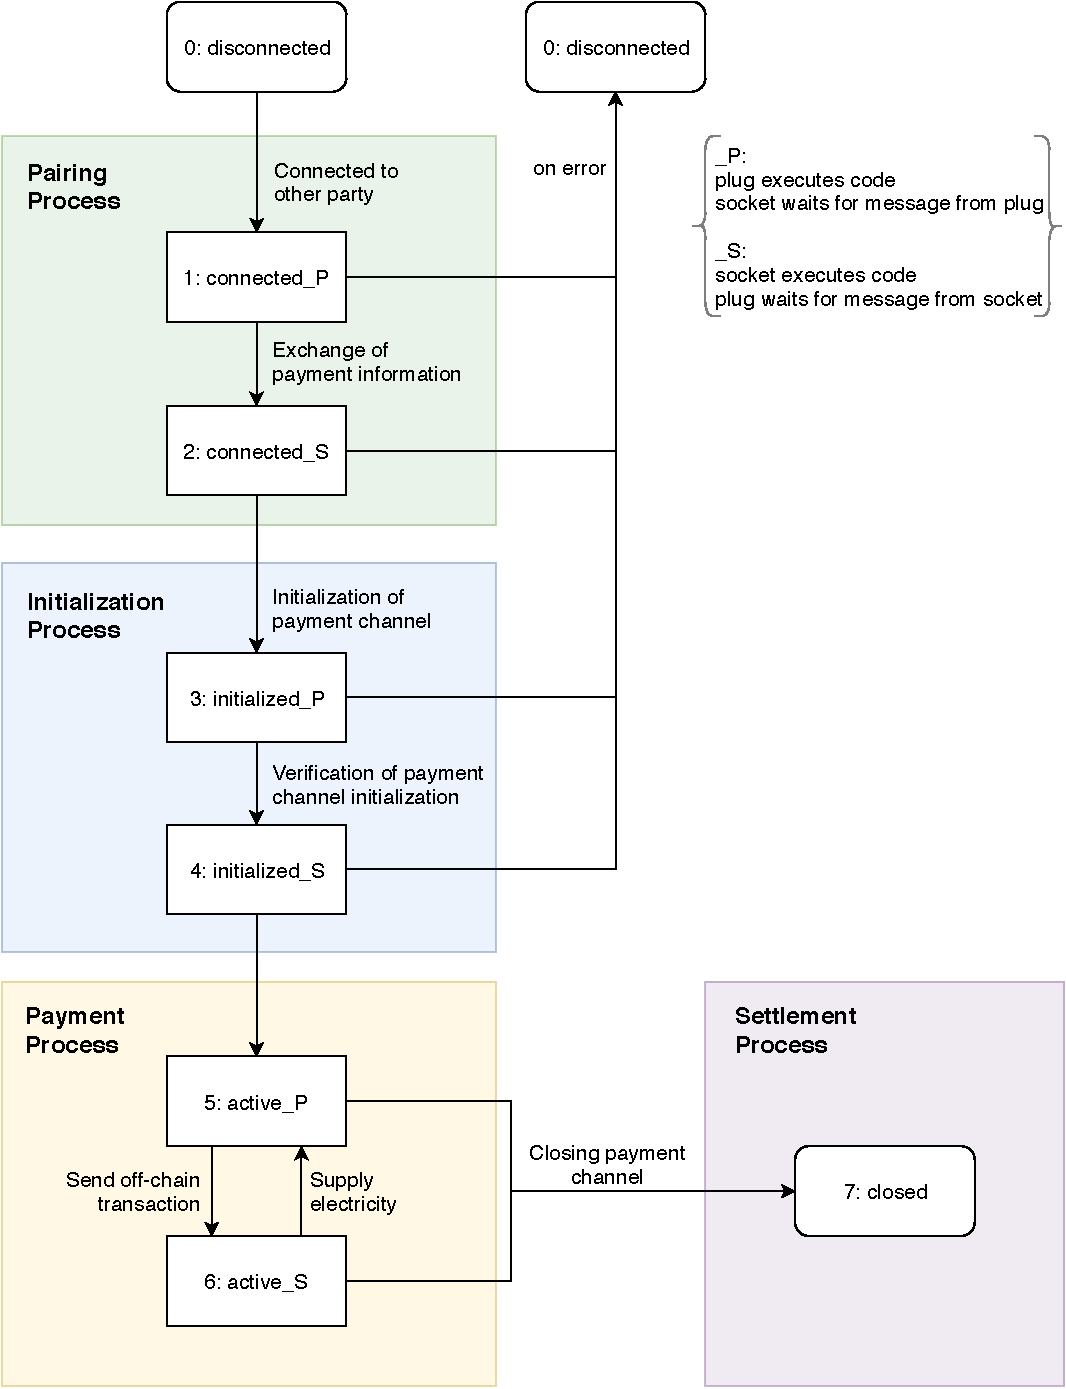
\includegraphics[height=15cm]{img/state_machine.pdf}
    \caption{Concept of the state machine}
    \label{fig:state_machine}
  \end{center}
\end{figure}
According to the different states, different code is executed  – the suffix \textit{\_P} means that the plug is currently executing code and the socket is expecting a message from the plug, \textit{\_S} means the opposite.
\\
During the pairing process, both parties exchange all required payment information with each other.
The payment channel is initialized and all payment information is verified by both parties in the initialization process.
During the third phase, the plug and the socket exchange off-chain transactions for electricity until any party wants to stop the payment process.
Then the settlement process is initialized closing the payment channel and finalizing the transactions on the blockchain.
\\\\\\

\textbf{Pairing Process}\\
The goal of the pairing process is to establish a connection between the customer and the supplier and exchange all necessary payment information.
\\
\begin{figure}[H]
    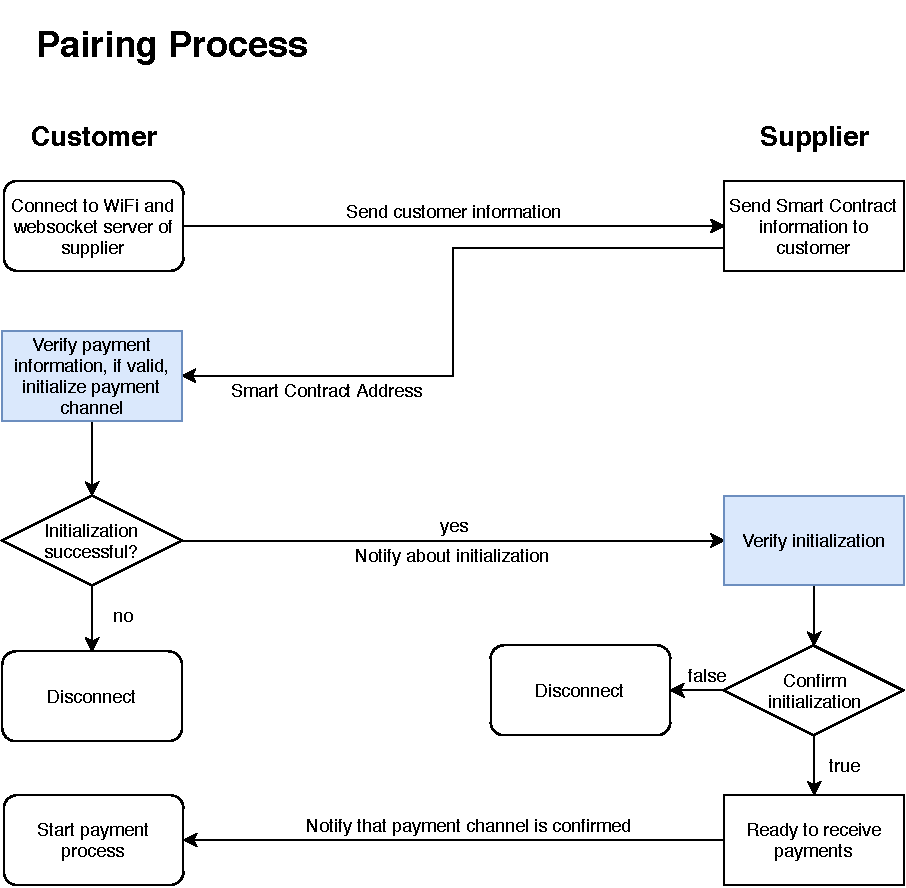
\includegraphics[width=\textwidth]{img/Plug-Socket-pairing_process.pdf}
    \caption{Pairing process}
    \label{fig:pairing_process}
\end{figure}
Both, the customer in form of the plug and the supplier in form of the socket start in the \textit{disconnected} state.
\\\\
As soon as a new customer connects to the socket and wants to purchase electricity, both parties transition to the \textit{connected\_P} state.
The socket now expects the customer information, in this case the Ethereum address, from the plug.
The address is important to know as it will be later used to verify off-chain transactions and whether the payment channel was initialized correctly.
\\\\
When the customer sends the required information, the plug and the socket enter the \textit{connected\_S} state.
The supplier can check the address against white- or blacklists and decide whether to accept payments from this address or not.
If the customer is accepted, the socket transfers the address of the smart contract, as it is required by the customer to fetch the rest of the payment information.
Both parties now enter the initialization process.
\\\\\\
\textbf{Initialization Process}\\
During the initialization process demonstrated in figure \ref{fig:verification_process} all the necessary payment information is fetched from the smart contract and the payment channel is initialized by the customer.
\\\\
Both parties start in the \textit{initialized\_P} state.
The plug is required to retrieve all relevant payment information which is stored in the smart contract, where it can be easily updated if necessary.
Payment information required for the transaction is the price per second and the payment interval to calculate the value of each off-chain transaction sent.
Optional payment information could be the owner of the smart contract, a minimum deposit value, minimum and maximum charging durations and the expiration date, depending on the implementation.
The plug should also verify that there is no other payment channel currently active.
\\
After the price was fetched from the smart contract, the customer can decide whether to accept the price and continue with the initialization process or to disconnect.
\\
If the price is accepted, an on-chain transaction is signed on the microcontroller and submitted to the Ethereum network.
This transaction calls a function inside the smart contract and initializes the payment channel.
A maximum amount of Ether that the customer is willing to spend during the charging process is passed alongside the smart contract call which will be deposited into the contract.
The customer now has to wait until the transaction was mined.
If the payment channel was initialized correctly, the socket is notified about the initialization and both devices enter the \textit{initialized\_S} state.
\\\\
If the socket can confirm that the payment channel was initialized correctly, it notifies the customer that it is ready to accept off-chain transactions and the payment process begins.
\begin{figure}[H]
    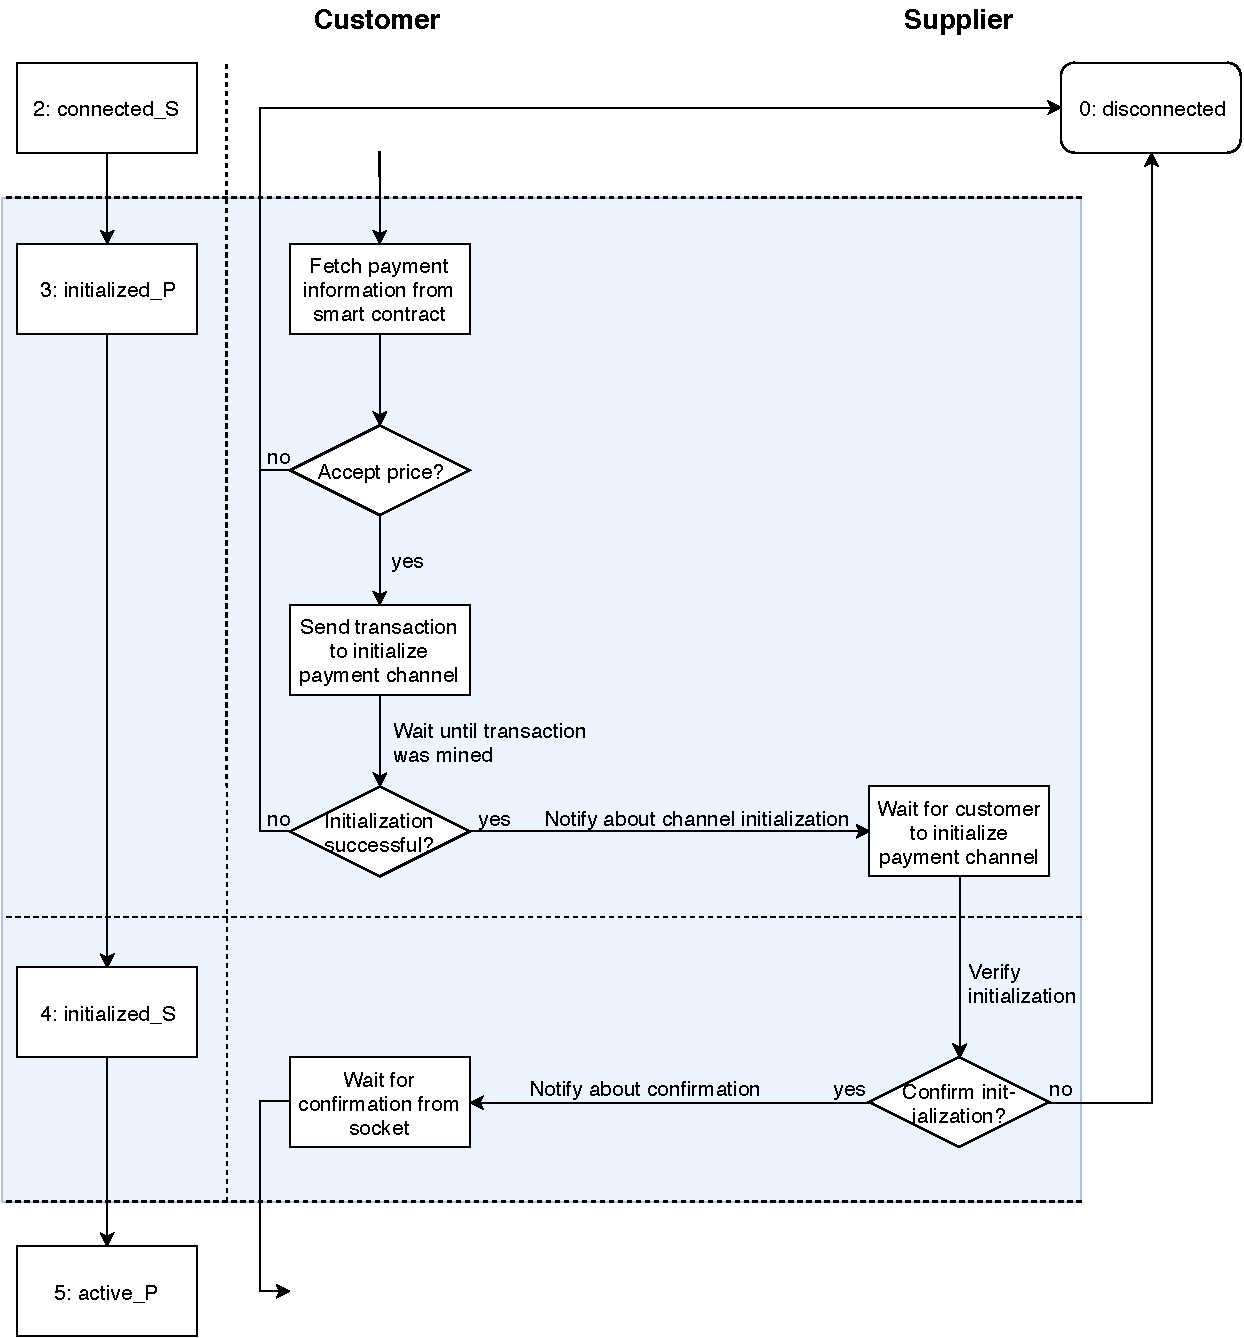
\includegraphics[width=\textwidth]{img/Plug-Socket-verification_process.pdf}
    \caption{Verification process}
    \label{fig:verification_process}
\end{figure}
\leavevmode
\newpage
\textbf{Payment Process}\\
The goal of the payment process is to exchange off-chain transactions for electricity.
\\
\begin{figure}[H]
    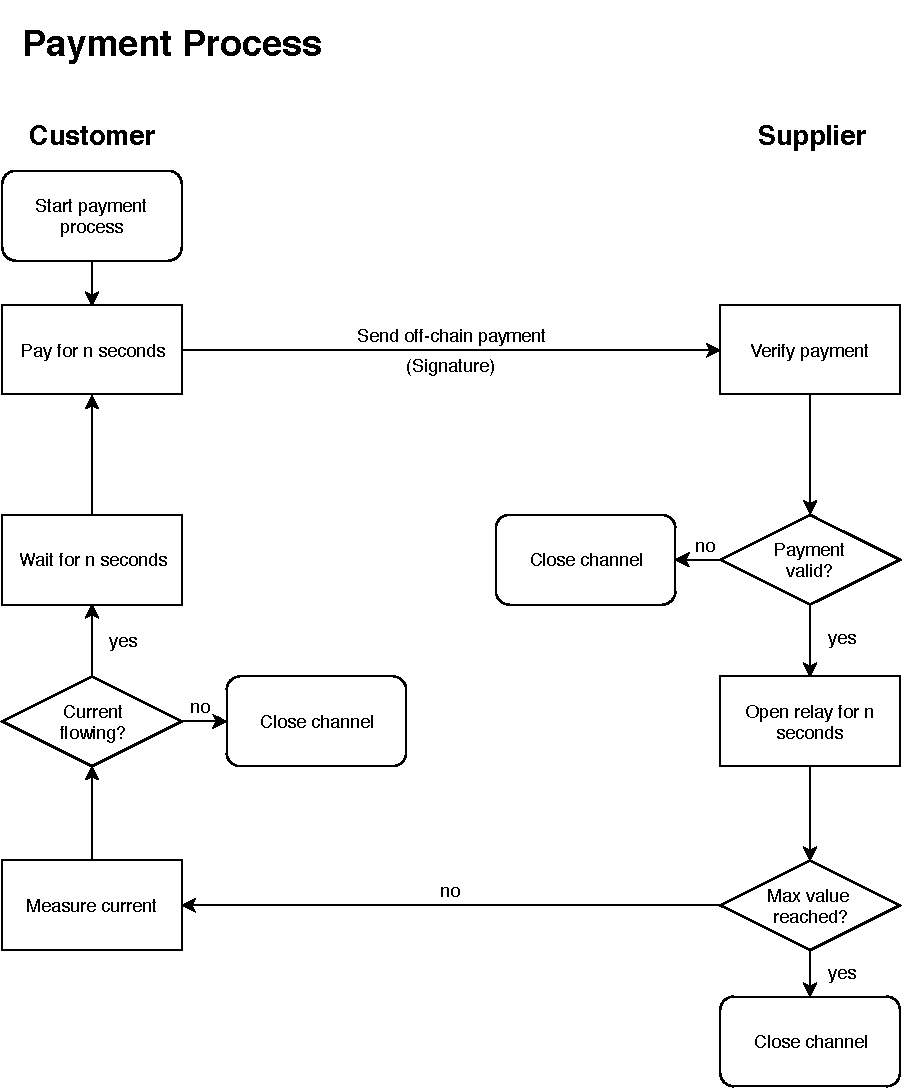
\includegraphics[width=\textwidth]{img/Plug-Socket-payment_process.pdf}
    \caption{Payment process}
    \label{fig:payment_process}
\end{figure}
The payment process starts when the customer sends the first off-chain transaction to the supplier.
As it would be really inconvenient for the socket to store and submit hundreds of off-chain transactions, only one signature can be submitted to the smart contract.
With every transaction the plug increases the value of the off-chain transaction.
Every signature is valid but it's in the interest of the supplier to submit the latest signature with the highest value.
The value of the transaction is calculated as follows:
\\
$value = number\_of\_transactions * price\_per\_second * seconds\_between\_transactions$
\\
With the assumed values from chapter 3 (a total price of 18 \euro{} over a duration of 11 hours) roughly 0.007 \euro{} are transmitted with each off-chain transaction.
With the formula above, this means that the value hashed and signed is 0.007 \euro{} for the first transaction, 0.014 \euro{} for the second, and so on.
As the smart contract operates on ETH and not \euro, the values are converted to Wei first.
\\\\
When the socket receives an off-chain transaction, it should verify that the payment is actually valid.
Both parties keep track of the number of transactions sent and know the price per second, therefore the data that was digitally signed by the customer can be recreated.
Using the data and the signature received from the plug the signer's Ethereum address can be recovered.
It should match the Ethereum address received during the pairing process for the transaction to be valid.
\\
If the off-chain transaction is valid, the microcontroller can open the relay for the specified amount of seconds, supplying the plug with electricity.
\\\\
To ensure that the socket doesn’t deliver more electricity than the plug can pay for, the supplier has to check whether the maximum value, that was deposited into the smart contract, was reached.
If that is the case, the channel is closed, ending the exchange of electricity.
\\\\
After the plug sends a transaction that pays for the specified amount of seconds, it should start measuring the current.
As soon as it is detected, the plug starts a timer and waits an appropriate amount of time to send the next transaction.
For the implementation, a new transaction is sent to the socket when there is 5 seconds of paid electricity left to ensure a steady flow without interruptions.
If the customer paid for electricity but no current is measured in return, it can immediately interrupt the payment process, by closing the payment channel, without losing another payment.
\\\\\\
\textbf{Settlement Process}\\
The settlement process closes the payment channel taking the value of the off-chain transactions and paying out the balances to each participant on the blockchain, finalizing the exchange.
\begin{figure}[H]
  \begin{center}
    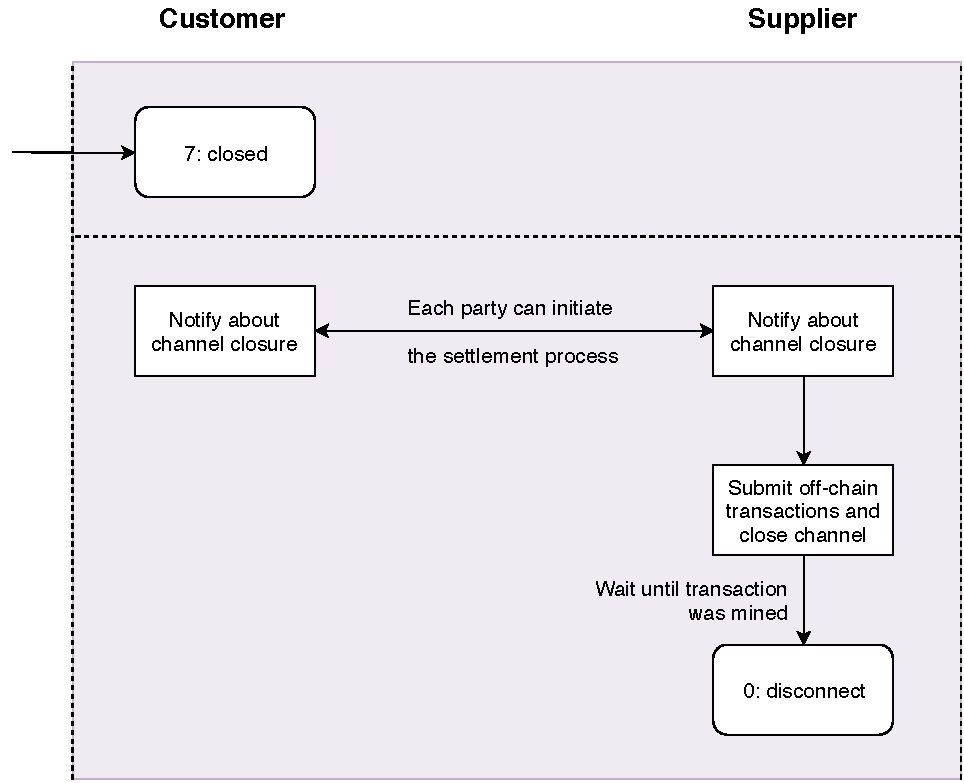
\includegraphics[height=9cm]{img/Plug-Socket-settlement_process.pdf}
    \caption{Settlement process}
    \label{fig:settlement_process}
  \end{center}
\end{figure}
As soon as a party wants to stop the payment process, e.g. when the battery of the customer is fully charged or the socket received an invalid signature, it can notify the other party about it.
The socket signs an Ethereum transaction which calls a function inside the smart contract, that takes the latest off-chain transaction, which contains the total value spent by the plug up to this point, as an argument.
The smart contract verifies the submitted signature and pays out the amounts accordingly.
\\
The smart contract also protects the customer, as it was mentioned before.
If the supplier fails to submit a valid signature in a certain amount of time and the payment channel expires, the deposited amount can be withdrawn again.
\\
\subsection{Transactions}
During the initialization, payment and settlement process transactions have to be sent by the plug and socket.
The following chapter will go into detail on how transactions were implemented for this thesis.
\\\\
When researching existing implementations of the generation of on-chain transactions for the Ethereum network on a microcontroller level, it was discovered that these implementations are far from production ready, as opposed to implementations with high level programming languages.
In an effort to find existing code that could be used as a foundation for the implementation some utility libraries were found, but many of them were not compatible with the microcontroller and the ones that were, often had to have issues fixed or additional functions implemented.
\\\\
Payment channels and off-chain transactions were implemented in this bachelor’s thesis as well.
They are a subset of state channels, which currently are a heavily researched topic on their own, therefore no standard exists that could be followed for the implementation.
As far as exploratory research went, every state channel implementation was still under development and not a single implementation of a payment channel on an embedded level could be found\cite{state-channels}.
Therefore an entire concept for the payment channel had to be developed, that could run independently on microcontrollers.
\\\\
The process of sending an on-chain transaction can be broken down into the following steps: 
\begin{enumerate}
    \item Gather data
    \item Encode data
    \item Hash data
    \item Sign hash
    \item Submit signature
\end{enumerate}
Off-chain transactions were implemented in a way to mimic the functionality of on-chain transactions.
The following chapters will go into detail of the implementation of on- and off-chain transactions, why certain design choices were made and which challenges were faced.
\\\\\\
\textbf{1. Gather Data}\\
The following information is necessary to send an on-chain transaction on the Ethereum blockchain:
\begin{enumerate}
  \item \textit{to}: Receiving address of the transaction.
  \item \textit{value}: Value of the transaction in Wei.
  \item \textit{data}: Hexadecimal data can be passed with the transaction.
  When sending a transaction to a smart contract, the data is used to define which function is called and to pass arguments.
  The first four bytes are the function identifier followed by the function arguments which are encoded according to the "abi specification"\cite{abi-encoding}.
  As the signature, which is a dynamic byte array, is passed to the smart contract alongside other variables, the encoding according to the specification had to be implemented.
  \item \textit{nonce}: The nonce is important, as it protects a user against replay attacks and guarantees that transactions are executed in the correct order.
  The nonce starts at zero and increments by one after a transaction was sent.
  This means that transactions, where the nonce is less than the total amount of transactions sent by the account, are rejected by the Ethereum network.
  Without the nonce an attacker could resubmit a transaction, that was already mined, over and over again to drain the balance of a victim.
  \item \textit{gas price}: The fee of a transaction that gets paid out to a miner in Wei.
  The higher the fee, the faster the transaction will be mined.
  The Rinkeby testnet uses a \abbr{Proof of Authority}{PoA} mining algorithm, which only allows a few accounts to act as miners, as in a test environment without monetary incentives, stability is more important than decentralization.
  Therefore there are no competing miners and high transaction fees are not relevant.
  A transaction with a gas price of 1~GWei will be usually included in the next block resulting in a confirmation time of less than 15 seconds.
  On the mainnet the gas price should be checked carefully, so the transaction is mined in a reasonable amount of time to not interfere with user experience.
  \item \textit{gas limit}: The gas limit specifies how much code can be executed with a transaction.
  The base limit of any transaction, whether it's a smart contract call or not, is 21,000 gas – it covers the storage of the transaction on the blockchain as well as the elliptic curve operation to recover the sender of the transaction\cite{design-rationale}.
  Each additional computational step costs more gas, e.g. an addition (opcode: ADD) costs 3 gas, loading a variable from storage (opcode: SLOAD) costs 200 gas and even goes as far as 20,000 gas if a storage value (variable stored on the blockchain) is set from zero to non-zero.
  As it can be seen, storing data on the blockchain is one of the most expensive operations to discourage storing vast amounts of information on-chain.
  If the gas limit is set too low and there is not enough gas to finish the smart contract execution, the transaction is unsuccessful and reverts any changes made.
  If the limit was set too high, any unused gas is refunded to the sender.
  Thus, when implementing smart contract calls on the microcontroller, it's important to provide enough gas for all computations.
  The total transaction fee is calculated by multiplying the gas price with the gas limit.
  \item \textit{chain ID}: Each Ethereum blockchain has a unique chain ID to differentiate between different chains.
  For example the mainnet uses the ID 1 and the Rinkeby testnet uses the ID 4.
  With the Ethereum Improvement Proposal 155 (EIP-155)\cite{eip-155} the chain ID should be included into a transaction to prevent so-called cross chain replay attacks, where a transaction on one Ethereum chain can be resubmitted to another Ethereum chain.
\end{enumerate}
\leavevmode
\\
Although the functionality of off-chain transactions mimic on-chain transactions, not every parameter listed above is required.
Because the payment channel was implemented between two parties only, the \textit{to} parameter can be left out.
The value, as demonstrated in the previous chapter, is defined as the total value spent up to a specific point in Wei and is included in the off-chain transaction.
There is no need to pass any data with the off-chain transactions, therefore no data is included.
No transaction fees are paid either, so the gas limit and gas price can be dropped from the off-chain transaction.
A nonce is mandatory to protect the customer. Without it, a supplier could just resubmit an off-chain transaction with a higher value from a previous exchange, stealing money from the customer. The smart contract keeps track of the nonce of each customer and needs to be fetched by both parties during the initialization process.
Although the \textit{chain ID} is not required to be included, a similar kind of attack can be conducted across different smart contracts.
If every socket has its own smart contract, an off-chain transaction with a higher value originally submitted on one smart contract, can be wrongfully resubmitted for a different exchange on another smart contract.
Therefore the address of the smart contract managing the payment channel is included inside the off-chain transaction.
\\\\\\
\textbf{2. Encode Data}\\
On-chain transactions are encoded with the \abbr{Recursive Length Prefix}{RLP}\cite{ethereum-yellow-paper}.
Before the data listed above is hashed, it's converted into hexadecimal and therefore byte-arrays.
The benefit of RLP encoding is that parameters of variable length are encoded in a way that all parameters can be extracted from the resulting byte array in the end.
This is mandatory so miners can extract the required data from the encoded byte array to fulfill the transaction.
RLP was especially designed for Ethereum to efficiently encode these values with the following rules: 
\begin{itemize}
  \item If a single byte is in the range of 0x00 and 0x7f, the byte is its own encoding.
  \item If a byte array is 0 to 55 bytes long, the byte array is prefixed with a single byte with the value 0x80 plus the length of the byte array.
  \item If a byte array is longer than 55 bytes, it's encoded by a first byte that has the value 0xf7 plus the length of the length prefix of the byte array, followed by the bytes describing the length of the byte array and finally the byte array itself.
  \item A list of byte arrays can be encoded as well, as it's required for the transaction data.
  All items are encoded individually first and then encoded again as a total byte array.
  This allows to encode data, no matter how nested the information is.
\end{itemize}
For the implementation, code from a RLP C++ library was used, which was written by Takahiro Okada\cite{rlp-lib}.
The following changes had to be made to the library so it could be used for the implementation.
\begin{itemize}
  \item The library had to be rewritten, to implement encoding of transactions into one utility library and to make it compatible with the microcontroller.
  \item The library now supports the EIP-155\cite{eip-155}, when encoding transactions with the chain ID.
  \item An wrong calculation was fixed that would incorrectly encode byte arrays longer than 55 bytes.
  \item The memory allocation of the library had to be adjusted, as it didn't allocate enough memory to handle all data that needed to be encoded for the transactions.
\end{itemize}
\leavevmode
\\
The smart contract validates an off-chain transaction by recreating the signed data and using it to recover the signers address from the signature.
As the nonce and the contract address are already stored inside the smart contract, only the value and the signature have to be passed to the smart contract function.
The Solidity smart contract programming language uses so-called encoding in packed mode before hashing as a standard\cite{packed-spec}:
\\
\begin{lstlisting}[language=Solidity, numbers=none]
abi.encodePacked(
  _value,
  contractAddress,
  customerNonce
)
\end{lstlisting}
\leavevmode
\newpage
To ensure consistency, the same encoding had to be implemented on the microcontrollers with the following rules:
\begin{itemize}
  \item all variables are converted to bytes and concatenated together
  \item "types shorter than 32 bytes are neither zero padded nor sign extended"\cite{packed-spec}
  \item "dynamic types are encoded in-place and without the length"\cite{packed-spec}
\end{itemize}
\leavevmode
\\\\
\textbf{3. Hash data}\\
The encoded data of both, on- and off-chain transactions, is hashed using the Keccak-256 hashing algorithm.
This algorithm is almost identical with the official SHA-3 implementation, but Ethereum uses Keccak-256 instead, which was "the winning entry to the SHA-3 contest"\cite{ethereum-yellow-paper}.
\\\\
Before signing a signature that is used on the Ethereum blockchain, e.g. an off-chain transaction, it's recommended that the data is prefixed with an Ethereum specific prefix\cite{prefix}.
The prefix makes the signature recognizable as an Ethereum specific signature and protects users from attackers letting them unknowingly sign a transaction, instead of a message.

The encoded data is hashed, then prefixed according to the following rules:
\\
"\textbackslash x19Ethereum Signed Message:\textbackslash n" + len(message) + message
\\
As a 256 bit hash is the message that is signed, the length of the prefix is always 32 bytes.
The prefixed message is then hashed again:
\\
\begin{lstlisting}[language=Solidity, numbers=none]
bytes32 message = keccak256(
  abi.encodePacked(
    value,
    contractAddress,
    customerNonce
  )
);

bytes32 prefixedMessage = keccak256(
  abi.encodePacked(
    "\x19Ethereum Signed Message:\n32",
    message
  )
);
\end{lstlisting}
The plug mirrors the smart contract implementation demonstrated above during the generation of off-chain transactions.
It needs to produce the same hash for the same input data as the smart contract to make it verifiable for the closure of the payment channel.
\newpage
\textbf{4. Sign data}\\
Although Ethereum relies on ECDSA elliptic curve signatures, there are some additional rules and features that differ the signature process from its standard implementation:
\begin{itemize}
  \item It takes up to 2 guesses to recover the public key / address from the $r$ \& $s$ values of an ECDSA signature.
  Therefore a third value $v$, also called the \textit{recovery ID} is calculated, that enables the immediate extraction of a public key from a signature.
  According to the Ethereum yellow paper\cite{ethereum-yellow-paper} "the recovery identifier is a 1 byte value specifying the parity and finiteness of the coordinates of the curve point for which r is the x-value".
  The recovery ID is determined during the signature process by looking at the y value on the elliptic curve with the following formula:
  \\
  $v = 27 + (y \% 2)$
  \\
  i.e. if y is even the recovery ID equals to 27, if it's odd, it equals to 28.
  The formula is used for signatures of all kinds.
  With the aforementioned EIP-155, optionally the following formula can be used for on-chain transactions, securing them against cross-chain replay attacks:
  \\
  $v = chain\_id * 2 + 35 + (y \% 2)$
  \\
  This means that for transactions on the Rinkeby network the recovery ID is either 43 or 44.
  For the generation of off-chain transactions the first and for on-chain transactions the second formula was implemented on the microcontrollers.
  \item According to the Ethereum yellow paper\cite{ethereum-yellow-paper} the $s$ part of the signature has to be less or equal than half of the numeric value of the elliptic curve $n$, which equals to 
  $0x7FFFFFFFFFFFFFFFFFFFFFFFFFFF
  \\FFFF5D576E7357A4501DDFE92F46681B20A0$
\end{itemize}
As a foundation, a standard implementation of the ECDSA algorithm\cite{micro-ecc} was used.
Both additional features of the Ethereum specific signatures had to be implemented extending the library.
\\\\
\textbf{5. Submit signature}\\
To submit an on-chain transaction, the transaction data and the signature has to be RLP encoded again.
The resulting byte array can then be submitted to the Ethereum network by sending the transaction to the node.
\\\\
As previously mentioned, both the plug and the socket, keep track of all transaction data themselves.
Therefore when the plug is paying for electricity with an off-chain transaction, it simply sends the signature to the socket.
\\\\\\
\textbf{Additional challenges}\\
Smart contracts mainly work with 256 bit unsigned integers for numbers, but most microcontrollers are not capable of working with integers this big.
When fetching a \textit{uint256} value from a smart contract, the value returns as a hexadecimal string from the node.
The largest fixed with integer type \textit{uint64\_t} or \textit{unsigned long long} can only store 64 bits of data which equals roughly 18.44 ETH.
If the value exceeds exceeds 64 bit, parsing, storing and calculating with the value becomes a lot more challenging, as the data has to be processed as a byte array.
\\\\
As all the communication with the Ethereum blockchain is processed through the node and http requests, all data is mostly handled as hexadecimal represented by char arrays.
These use more space than byte arrays.
During the entire process of generating on-chain transactions, the data for the smart contract call has to be encoded, then encoded with the rest of the transaction data, hashed, signed and the resulting signature has to be encoded with the transaction data again.
The generated transaction then has to be put into a JSON http request body and the response that returns from the node has to be JSON parsed to receive required data.
This generates a lot of data mainly in the form of char arrays which can get long, depending on the arguments passed to a smart contract.
On an embedded platform with limited memory a lot of optimization and memory management is required to successfully generate a transaction.
\\\\
\subsection{Smart Contract}
Security is extraordinarily important for smart contract development, as possibly large sums of money are handled and the code is immutable, and can’t be changed once the smart contract has been deployed to the Ethereum network.
This chapter will go over the smart contract implementation, some security best practices and design choices.
The entire source code can be found under the appendix, listing \ref{lis:safemath} \& \ref{lis:pc_sc}.
\\\\
The smart contract was designed that only one contract is responsible for one socket which can only handle one payment at the time.
One of the most important rules for smart contract development is to keep the code as simple as possible.
Adding complexity only increases the risk of a critical issue.
When the customer initializes the payment channel, a maximum transaction value is deposited which is kept inside the smart contract until the channel is closed or expires.
Additionally the address of the customer is stored inside the smart contract as a global variable which will be used to verify the off-chain transactions:
\begin{lstlisting}[language=Solidity, numbers=none]
// set channel customer to the address of the caller of the transaction
channelCustomer = msg.sender;
\end{lstlisting}
\leavevmode
\\
The channel can be timed out by any participant on the network after the expiration date has been reached, returning the deposited funds to the customer.
The function to close the channel can only be called by the supplier.
The total transaction value and the signature of the final off-chain transaction is passed to the function as an argument.
From the three values inside the off-chain transactions, the transaction data is regenerated.
The nonce and the address of the smart contract cannot be forged, as these values are not passed by the supplier.
Instead they are taken directly from the storage of the smart contract itself.
The smart contract repeats the same steps to generate the transaction data as the plug – the data is hashed and prefixed with the Ethereum specific prefix:
\\
\begin{lstlisting}[language=Solidity, numbers=none]
bytes32 message = keccak256(
  abi.encodePacked(
    // value passed as an argument
    _value,
    // variable to receive the smart contract address
    address(this),
    // gets the nonce of the current channel customer
    customerNonces[channelCustomer]
  )
);

bytes32 prefixedMessage = keccak256(
  abi.encodePacked(
    "\x19Ethereum Signed Message:\n32",
    message
  )
);
\end{lstlisting}
\leavevmode
\\
The resulting \textit{prefixedMessage} should result in the same data that the customer used to sign the off-chain transaction.
Solidity offers a function to recover the address of the signer, if provided with the signed data and the signature.
\\
\begin{lstlisting}[language=Solidity, numbers=none]
return ecrecover(prefixedMessage, v, r, s) == channelCustomer;
\end{lstlisting}
\leavevmode
\\
This function returns true if the recovered address matches the current payment channel customer.
The verification of the off-chain transaction is tamper proof.
If the supplier tried to provide a false value with the signature, the recreation of the data would result in data that the customer did not sign.
Therefore the \textit{ecrecover} function would return an address that does not match the current channel customer.
Only the correct data both parties agreed to can be used to close the payment channel.
\\\\
If the signature was valid, the nonce of the customer increments by one, making all off-chain transactions up to this point invalid.
Then the transaction value is paid out to the supplier and the rest is refunded to the customer, closing the payment channel.

\subsubsection{Best practices}
The smart contract implements the so-called pull over push method\cite{best-practice}.
When closing the payment channel, the according transaction values could be immediately paid out to the customer and the supplier.
An attacker could write a smart contract that would initialize a payment channel and would always revert the transaction when it received Ether during the settlement.
In this case the payment channel would be locked forever, as the customers balance could be never paid out.
Instead a balance variable is used, from which each party can withdraw their share without the risk of blocking the smart contract.
\\\\
Solidity has no built in checks for integer under- and overflows, which can become a major security issue, especially when dealing with balances, allowing an attacker to drain a smart contract.
A so-called SafeMath library, as the one found under appendix \ref{lis:safemath} can help in preventing integer under- and overflows.
\\\\
Another security concern that comes up when withdrawing Ether from balances is the reentrancy attack.
In traditional programming, an amount would be paid out and upon success, the balance would be adjusted to reflect the new balance.
In smart contract programming this practice resulted in a hack where an attacker recursively withdrew the balance from a smart contract, resulting in theft of over 3.6 million ETH, which is worth 792 million \euro{} at the time of writing\cite{dao-hack}.
Therefore it's very important to set the new balance before transferring Ether.
If the transfer fails, the entire smart contract call is reverted, so the new balance only comes into effect if the transaction was successful.